\documentclass[11pt,a4paper]{book}
\usepackage[italian]{babel}

\usepackage{acronym}
\usepackage{graphicx}
\usepackage{amsmath}
\usepackage{amsfonts}
\usepackage{amssymb}
\usepackage{psfrag}
\usepackage{listings}
\usepackage{url}
\usepackage{setspace}
\usepackage{cmap}
\usepackage{hyperref}
\hypersetup{
    colorlinks,%
    citecolor=black,%
    filecolor=black,%
    linkcolor=black,%
    urlcolor=black
}

\begin{document}


%----------------------------------------------------------
%	Fronte - Sommario - Varie
%----------------------------------------------------------
%!TEX root = ../tesi.tex
\tableofcontents
\listoffigures
%\listoftables
%!TEX root = ../tesi.tex
\chapter*{Acronimi}

\begin{acronym}[GPGPU]

	\acro{SF}{Shadow Framework}
	\acro{GPU}{Graphic Processing Unit}
	\acro{UML}{Unified Modeling Language}
	\acro{fps}{frame per secondo}
	\acro{API}{Application Programming Interface}
	\acro{GPGPU}{General-Purpose computing on Graphics Processing Units}
	\acro{kB} kilobyte
	\acro{MB} megabyte
\end{acronym}



%----------------------------------------------------------
%	Capitoli
%----------------------------------------------------------
%!TEX root = ../tesi.tex

\chapter{Introduzione}
\label{ch:introduzione}
Questo progetto di tesi \`e stato realizzato nell'ambito dello sviluppo dello \ac{SF} 2.0, un framework per lo sviluppo di applicazioni che fanno uso di grafica tridimensionale real-time ideato e sviluppato dall'Ingegner Alessandro Martinelli.

La grafica tridimensionale, o computer grafica 3d, consiste nell'utilizzo di modelli geometrici tridimensionali da parte di un computer per il calcolo e il rendering\footnote{Con rendering, in computer grafica, si intende il processo che attraverso l'elaborazione di un modello determina il colore di ogni pixel contenuto in una immagine digitale.\cite{wiki:rendering-it,wiki:rendering-en}} di immagini digitali.
Essa \`e attualmente molto diffusa ed utilizzata in moltissimi campi, cosa che l'ha resa un'esperienza comune nella vita di tutti i giorni, non solo infatti ne viene fatto un uso intensivo nella pubblicit\`a e nell'intrattenimento, ma anche in campi come la medicina e la ricerca scientifica.

La grafica tridimensionale real-time \`e un ramo specifico della grafica tridimensionale che si focalizza sulla generazione di simulazioni di ambienti e/o oggetti con la quale un utente pu\`o interagire osservando una reazione coerente nella simulazione. Questo senso di interazione viene fornito da una generazione sequenziale di immagini che come nelle pellicole cinematografiche danno un'illusione di movimento, ma in cui l'effettivo contenuto dei fotogrammi non \`e predeterminato ed \`e calcolato al momento sulla base degli input forniti.

In base a quanto esplicato in \cite{book:realtimerendering}, per poter avere un'interazione soddisfacente \`e molto importante che la velocit\`a con cui vengono visualizzate le immagini, misurata in \ac{fps}, si mantenga stabile ed il pi\`u possibile elevata in modo da minimizzare i tempi di risposta ed impedire che questi interferiscano con l'interazione stessa.
Ci\`o pone il problema di ottenere un alto valore di \ac{fps} che a sua volta implica dei vincoli temporali sulla possibile elaborazione dei modelli tridimensionali: se infatti si volesse mantenere una velocit\`a di visualizzazione pari a 60 \ac{fps}, il tempo di calcolo a disposizione per l'elaborazione di un frame rispetto al precedente ammonta a circa 15 millisecondi.
Questa caratteristica differenzia profondamente la grafica real-time da quella non-real-time in cui, non avendo vincoli temporali stretti per la generazione dei frame, il focus \`e invece spostato sull'applicazione di modelli di elaborazione complessi e computazionalmente onerosi che siano in grado di generare immagini il pi\`u fotorealistiche possibile. 

Le problematiche della grafica real-time hanno imposto nel corso degli anni lo sviluppo di tecniche e tecnologie specifiche di settore il cui stato dell'arte \`e oggi rappresentato dall'ultima generazione di \ac{API} di programmazione grafica, dalle \ac{GPU}\footnote{Una \ac{GPU} \`e un microprocessore dedicato alla generazione delle immagini visualizzate sullo schermo di un dispositivo, alleggerendo da questo carico il processore principale.} a pipeline programmabile e dai Linguaggi di Shading.

Queste tecnologie hanno assunto una grande importanza perch\'e non solo consentono di raggiungere elevatissimi livelli di qualit\`a e prestazioni quando sono utilizzate per la generazione di grafica 3D real-time, ma la ricerca su di esse ha portato allo sviluppo del \ac{GPGPU} ovvero la possibilit\`a di utilizzare la capacit\`a di calcolo delle \ac{GPU} per processare anche dati differenti da quelli grafici.

Le \ac{GPU} a pipeline programmabile, in contrapposizione a quelle con pipeline fissa, permettono di adattare gli stadi della pipeline di renderizzazione mediante l'utilizzo dei linguaggi di Shading. In sostanza l'hardware viene programmato per il calcolo di algoritmi specifici da applicare ai dati grafici. Ci\`o consente di adattare il processo di renderizzazione agli effetti che si desidera ottenere e di sfruttare l'hardware della \ac{GPU} per velocizzarne la computazione. Questo paradigma si \`e rivelato molto efficace ed efficiente, tanto che esso viene oggi applicato nella quasi totalit\`a delle \ac{GPU} moderne, sia che si tratti di dispositivi di fascia alta che di processori grafici dedicati ad architetture mobile come i cellulari.

Parallelamente le \ac{API} di programmazione grafica moderne si sono sviluppate consentendo lo sfruttamento sempre pi\`u efficiente delle risorse hardware delle \ac{GPU}, ma non solo: la loro integrazione su piattaforme software pensate per il mercato embedded ha consentito di osservare una proliferazione di applicazioni che fanno uso di grafica tridimensionale sia su cellulari che tablet. Per questi dispositivi, dotati ormai quasi obbligatoriamente di fotocamera, non \`e difficile trovare applicazioni di realt\`a aumentata che sfruttino le \ac{API} per inserire elementi grafici tridimensionali nelle immagini catturate dal sensore ottico. Un evento che nei prossimi anni avr\`a probabilmente un impatto molto significativo nel mercato, consiste nel fatto che molti sviluppatori di browser per la navigazione di internet stanno attualmente lavorando per integrare l'\ac{API} grafica WebGL all'interno dei loro software tramite JavaScript. Questo consentir\`a l'esecuzione di applicazioni 3D direttamente all'interno dei browser stessi, eliminando la transizione tra contenuti 3D e contenuti non-3D e consentendo una integrazione diretta con servizi internet di terze parti.

Di pari passo, i produttori di middleware, engine e framework\footnote{Nel contesto delle applicazioni per la grafica tridimensionale con middleware di solito si intendono componenti software dedicate a compiti specifici, come la gestione della fisica o il pathfinding, che vengono affiancate agli engine ed ai framework. Per una descrizione di cosa si intende per engine e framework e le differenze fra loro, fare riferimento alla sezione \ref{sec:panoramicastrumenti}} per applicazioni di grafica, hanno integrato nelle funzionalit\`a dei loro prodotti la capacit\`a di sfruttare le pipeline programmabili e tool per testare e comporre nuovi shader\footnote{Uno shader \`e un programma scritto con un linguaggio di shading, che viene caricato ed eseguito in hardware da una \ac{GPU}.}. Una sempre maggiore quantit\`a di queste case produttrici supportano le piattaforme mobile (come Android e iOS) e rilasciano plugin o applicazioni ``WebPlayer'' per distribuire contenuti attraverso i browser web. 
In alcuni casi, come quello citato in \cite{site:mozillaunrealannounce}, produttori di browser e case di sviluppo collaborano per migliorare le prestazioni di WebGL e convertire in JavaScript gli engine e i framework cos{\`\i} da poterli eseguire direttamente all'interno delle pagine web.

In questo contesto si inserisce lo Shadow Framework, il quale \`e stato progettato non solo per utilizzare e supportare tutte le tecnologie che costituiscono lo stato dell'arte nel campo della grafica 3D real-time, ma anche con l'obbiettivo di farlo sperimentando un nuovo approccio nella generazione e nella gestione dei dati grafici tridimensionali. La chiave di questo approccio consiste nell'abbandonare la vecchia concezione per cui gli oggetti tridimensionali sono scolpiti generando mesh di vertici che compongono triangoli, ma utilizzare primitive parametriche pi\`u complesse per poi sfruttare le capacit\`a delle pipeline programmabili e far generare dall'hardware stesso le mesh di punti necessarie per il processo di renderizzazione.
Questo tipo di procedimento permette di adattare la qualit\`a  del risultato visivo finale in base alle prestazioni dell'hardware a disposizione, eliminando la necessit\`a di produrre diverse versioni dello stesso modello la cui unica differenze consiste nel numero di vertici. \`E infatti sufficiente programmare la pipeline per produrre un minor numero di vertici per alleggerire il calcolo, mantenendo inalterato il modello parametrico di partenza.

Oltre hai vantaggi descritti, l'utilizzo di primitive parametriche permette di produrre file di dimensione molto contenuta rispetto ai sistemi classici in cui i file contengono l'elenco dei vertici che descrivono l'oggetto. Lo stesso paradigma viene usato all'interno del framework non solo per i modelli 3D, ma anche per la generazione delle texture da applicarvi, garantendo un meccanismo per scalarne la qualit\`a in base alle esigenze.

Sebbene una descrizione pi\`u dettagliata delle caratteristiche del framework venga fornita nel capitolo \ref{ch:shadowframework} vale la pena citare alcune delle sue caratteristiche salienti come: 
\begin{itemize}
	\item  la possibilit\`a di definire nuove primitive grafiche con un linguaggio specifico del framework;
	\item  la grande portabilit\`a: la versione di riferimento \`e sviluppata in linguaggio Java, ma \`e in corso di realizzazione un porting in C++ (iOS);
	\item  il design web-oriented: i meccanismi interni sono stati progettati per supportare l'utilizzo di dati in remoto ed \`e in corso di realizzazione una versione del framework in JavaScript;
\end{itemize}

%
% TODO: DA RIVEDERE, deve essere chiaro che l'applicativo voluto deve essere orientato al web
%
\section{Obbiettivo del progetto}
\label{sec:obbiettivo}
L'obbiettivo del progetto di tesi nasce dall'idea di produrre un'applicazione dimostrativa delle funzionalit\`a di rete offerte dallo Shadow Framework.
Ci\`o che si voleva ottenere era una coppia client-server in cui il server fosse in grado di gestire connessioni simultanee da parte di un numero indefinito di client. 
Ogni client, ottenuta una connessione con il server, doveva assere in grado di visualizzare una scena iniziale navigabile, richiedendo solamente i dati relativi all'ambiente in prossimit\`a di un eventuale avatar.
Successivamente si voleva analizzare due possibili approcci: uno in cui, secondo le necessit\`a, il client avrebbe richiesto al server i dati aggiuntivi riguardo la scena, ad esempio una volta raggiunti i bordi dell'ambiente, oppure un secondo in cui il server, comunicando attivamente con il client, tiene traccia degli spostamenti nella navigazione e fosse in grado di comporre in modo dinamico dei pacchetti di dati prevedendo le necessit\`a del client.

Le astrazioni del layer dati del framework sono state progettate specificatamente per consentire lo sfruttamento della comunicazione di rete, ma fino a quel momento non era stata fatta alcuna specifica implementazione che la utilizzasse. Si desiderava perci\`o produrre questo tipo di applicazione anche per individuare e correggere i probabili bug presenti nel codice dovuti a vincoli di sincronizzazione non evidenziati dai test effettuati con dati sulla macchina locale.

L'obbiettivo della tesi \`e cos{\`\i} diventato quello di produrre dei moduli di libreria che fossero utili allo sviluppo di applicazioni client-server.

La progettazione di questi moduli si \`e focalizzata su alcuni punti cardine che rappresentano la chiave dell'aspetto di sviluppo legato al progetto. Dato che la struttura del framework \`e ideata con l'obbiettivo di essere fortemente estendibile, \`e stato di fondamentale importanza utilizzare all'interno dei moduli i meccanismi e le astrazioni previste in tal senso e lo sviluppo dei moduli stessi \`e stato a sua volta guidato dai principi di estendibilit\`a e riutilizzo del codice.

% \section{Considerazioni generali}
% \label{sec:considerazioni}
% MENZIONARE I TEST

% Sulla base degli obbiettivi di progetto e a quanto che viene esposto successivamente nei capitoli \ref{ch:shadowframework} e \ref{ch:gestionedati}

% TODO: decidere su non avere il paragrafo

% Qui si pu\`o fare un discorso sulle parti del framework su cui \`e necessario focalizzarsi facendo riferimenti ai capitoli 2 e 3.

\section{Organizzazione del documento}
\label{sec:orgtesi}
Il presente documento \`e organizzato secondo la seguente suddivisione in capitoli:
\begin{itemize}
	\item  \textbf{Capitolo \ref{ch:shadowframework}:} in cui viene presentata una panoramica generale sullo Shadow Framework 2.0 in rapporto al panorama generale sui framework di programmazione di grafica tridimensionale real-time.
	\item  \textbf{Capitolo \ref{ch:gestionedati}:} in cui \`e descritta l'astrazione di gestione dei dati interna al framework e come essa viene utilizzata dalle applicazioni \ac{SF}.
	\item  \textbf{Capitolo \ref{ch:sfremoteconnection}:} in cui viene descritto il progetto Sf-Remote-Connection, i moduli che lo compongono, le funzionalit\`a offerte e i package java prodotti..
	\item  \textbf{Capitolo \ref{ch:testerisultati}:} in cui sono presentate le applicazioni di test ed i risultati prodotti.
	\item  \textbf{Capitolo \ref{ch:conclusioni}:} in cui viene presentato un riassunto del lavoro svolto, i risultati e vengono proposti alcuni sviluppi futuri.
\end{itemize}



%!TEX root = ../tesi.tex

\chapter{Lo Shadow Framework 2.0}
\label{ch:shadowframework}
Questo capitolo presenta inizialmente una panoramica sugli attuali sistemi per la realizzazione di applicazioni che fanno uso di grafica tridimensionale real-time. Successivamente viene presentato lo ShadowFramework 2.0, le sue caratteristiche, la sua struttura e i suoi sviluppi futuri.

% TODO: decidere se descrivere anche l'evoluzione rispetto alla precedente versione

\section{Titolo provvisorio}
\label{sec:titolo_provvisorio}
Lo scopo della presente tesi di laurea \`e quello di produrre dei moduli di estensione per lo Shadow Framework utili alla realizzazione di applicativi 3D orientati al web. 
Per lo stesso scopo esistono sul mercato una grande quantit\`a di soluzioni le cui caratteristiche possono essere notevolmente differenti in base al target di sviluppo a cui si rivolgono.

Prima di fornire una descrizione di alcune di queste soluzioni \`e bene introdurre alcuni concetti utili a comprendere quali sono i punti focali che distinguono un prodotto da un altro. L'elemento fondamentale di ognuno di questi questi software \`e l'\textbf{engine}, altrimenti detto rendering engine o 3D-engine. Questo \`e il nucleo di ogni programma grafico e fornisce una serie di meccanismi che, sfruttando le \ac{API} di programmazione grafica, permettono di disegnare su schermo i modelli tridimensionali voluti. Quando un prodotto consiste nel solo engine viene fornito nella forma di una libreria che permette permette di interagire con esso e configurarlo.

Dato che la pi\`u grande fetta di mercato per queste soluzioni software proviene dallo sviluppo di videogames sono nati una serie di software definiti \textbf{game engine}, questi sono veri e propri framework per la produzione di applicazioni 3D e, oltre al rendering engine, integrano al loro interno moduli per la gestione della fisica, del suono, delle animazioni e di tutte quelle componenti utili per lo sviluppo di giochi per computer. Questi framework possono essere forniti sia sotto forma di libreria da integrare nel proprio codice che con tool grafici che permettono di creare la propria applicazione da zero, utilizzando solamente gli strumenti forniti.

Seguendo questa classificazione e dato che l'intento dello Shadow Framework \`e fornire un set di librerie completo per la creare applicazioni grafiche, con moduli per gestire animazioni e dati oltre che alla semplice renderizzazione, senza per\`o vincolare all'utilizzo di librerie specifiche per elementi come l'intelligenza artificiale, il suono o altro che non sia direttamente coinvolto nella gestione della grafica, esso si trova a met\`a strada tra un rendering engine puro e un game engine.

Vengono ora presentati alcuni dei prodotti presenti sul mercato, la scelta di quali di essi presentare rispetto ad altri che non verranno citati non riflette la loro qualit\`a, ma sono stati scelti in base rappresentativa.

% TODO: inserire i simboli di copyright ecc
\subsection{Game engine per Adobe Flash}
In questo caso invece che un prodotto specifico si preferisce citare una categoria di software. Per l'ambiente di Adobe esistono una grande quantit\`a di game engine che sfruttano le \ac{API} Flash per effettuare il rendering dei contenuti. Sebbene questo framework venga utilizzato da molti anni per la realizzazione di applicativi e che per lungo tempo abbia rappresentato l'ambiente di riferimento per applicativi web 3D, solo dalla release 11 comincia a sfruttare l'accelerazione hardware per la grafica tridimensionale.

Attualmente l'accelerazione consente di sfruttare le GPU a pipeline programmabile, ma non consente di usare le modalit\`a legacy a pipeline fissa. 
Inoltre non vengono rese disponibili le \ac{API} grafiche per la programmazione nativa come OpenGL o DirectX, ma una \ac{API} proprietaria di nome Stage3D che fornisce un'astrazione di livello pi\`u alto e semplifica la gestione delle risorse.
Questo sebbene consenta di semplificare e unificare tutte le piattaforme compatibili rende necessarie delle limitazioni per conservare la compatibilit\`a, rendendo inaccessibili le funzionalit\`a pi\`u avanzate degli hardware moderni (ad esempio \`e supportato lo Shader Model solo fino alla versione 2.0 sebbene oggi sia disponibile la versione 5.0).
Questi dati sono reperiti da \cite{site:adobestage3d}.

\subsection{Unity 3D}
Unity 3D \`e un game engine completo che dal 2005 ad oggi ha accresciuto molto la sua popolarit\`a. Uno dei maggiori punti di forza di questo ambiente consiste nella presenza di una discreta quantit\`a di tool grafici integrati tra loro, per il controllo del workflow di sviluppo. Sono inoltre integrati molti moduli per controllare aspetti quali le animazioni, la verifica delle performance ed il networking.
Un qualit\`a di primo piano \`e la compatibilit\`a di un elevato numero di piattaforme, consentendo di pubblicare le applicazioni realizzate su piattaforme mobile (android e iOS), desktop (Windows, Mac e Linux), console e web (via browser).
A proposito di quest'ultimo caso la fruizione dei contenuti via web \`e effettuata con due diversi metodi: o tramite un player flash o tramite l'\ac{API} Google Native Client del browser Chrome che permette l'esecuzione di codice nativo all'interno del browser.
In generale Unity 3D \`e un game engine moderno con pieno supporto alle ultime tecnologie grafiche rendendolo uno prodotto molto rappresentativo.
Oltre alle caratteristiche citate buona parte del suo successo \`e probabilmente dovuto alla grande comunit\`a di sviluppatori, anche indipendenti, ed alla numerosa quantit\`a di asset grafici disponibili.

% \begin{figure}
% \begin{center}
% 
\includegraphics[width=3cm]{Immagini/Unreal_Engine_3_logo}
% 
\includegraphics[width=5cm]{Immagini/logo_unigine}
% \caption{Logo dell'Unreal Engine. Unreal, Unreal Engine, Unreal Technology, the Unreal Technology logo, and the Circle-U logo are trademarks or registered trademarks of Epic Games, Inc., in the United States of America and elsewhere. Other brands or product names are the trademarks of their respective owners. \label{f:unreallogo}} 
% \end{center} 
% \end{figure}

\subsection{Unreal Engine e Unigine engine}
Entrambi questi prodotti sono game engine completi piuttosto famosi per l'elevatissima qualit\`a delle loro capacit\`a di rendering. Entrambi vengono infatti spesso utilizzati come benchmark per testare le capacit\`a grafiche hardware. Entrambi questi progetti sono maturi e moderni essendo dotati di tool grafici specifici e supportando le pi\`u recenti architetture grafiche. Entrambi supportano la maggior parte delle piattaforme desktop, mobile e consolle. Sebbene L'Unreal engine supporti anche flash e L'Unigine no, sono presentati insieme in quanto esempio di nuovo approccio alla distribuzione via web: entrambe le compagnie produttrici di questi software stanno infatti investendo nel portare i loro framework a supportare \ac{API} WebGL. Gli annunci ufficiali possono essere trovati a questi riferimenti \cite{site:mozillaunrealannounce,site:unigineannounce}.



\section{Struttura dello Shadow Framework 2.0}
\label{sec:sfstructure}
%!TEX root = ../tesi.tex

\chapter{Gestione dei dati nello Shadow Framework 2.0}
\label{ch:gestionedati}

% TODO: ampliare l'introduzione
La gestione dei dati \`e un compito molto importante all'interno del framework. Attraverso l'utilizzo di un layer di gestione dati astratto, ogni mudulo del framework pu\`o essere salvato e caricato da file o trasferito attraverso un qualsiasi flusso di dati.
In questo capitolo viene presentata l'astrazione utilizzata dallo Shadow Framework nella gestione dei dati, le funzionalit\`a messe a disposizione ed i principali package e moduli coinvolti.

\section{Dati grafici}
\label{sec:dati grafici}
Data la natura del framework la tipologia di dato pi\`u critica e importante \`e quella che descrive le informazioni grafiche. 
L'unit\`a base di ogni dato di tipo grafico \`e l'\texttt{SFDataAsset}, questa \`e una classe astratta generica che serve ad automatizzare il processo di costruzione dei dati e inizializzazione degli stessi nella memoria grafica. Questo processo non pu\`o per\`o essere effettuato in qualsiasi momento, ma deve essere correttamente sincronizzato con il processo di rendering della pipeline del framework, in caso contrario i dati potrebbero venir alterati durante il disegno della scena portando ad effetti inaspettati.

\begin{figure}
\begin{center}
\includegraphics[width=\textwidth]{Immagini/sequenzaDataAsset}
\caption{Diagramma di sequenza della fase di costruzione di un SFDataAsset.\label{f:seqdataasset}} 
\end{center} 
\end{figure}

Il diagramma della figura \ref{f:seqdataasset} mostra la sequenza di operazioni necessarie affinch\'e le informazioni del DataAsset grafico vengano costruite correttamente e inizializzate nella memoria grafica in modo sincrono con il processo di rendering, gestito dal frame grafico \textbf{SFDrawableFrame}. Partendo da in alto a sinistra l'applicazione richiede la risorsa all'\texttt{SFDataAsset}, questo la costruisce con il metodo \texttt{build()} e notifica all'\texttt{SFInitiator} che la risorsa necessita di essere inizializzata nella memoria grafica tramite la chiamata \texttt{addInitiable()}, dopo di che il riferimento alla risorsa viene restituito all'applicazione.
Il processo di rendering chiede all'Initiator, ciclicamente e nel momento opportuno, di inizializzare nella memoria grafica tutti i DataAsset che sono in attesa di farlo. L'Initiator richiama allora il metodo \texttt{init()} di tutte le risorse in attesa di inizializzazione.
Questo procedimento assicura che tutte le risorse necessarie al processo di rendering siano inizializzate correttamente prima di essere usate.

\begin{figure}
\begin{center}
\includegraphics[width=\textwidth]{Immagini/sequenzaUpdatable}
\caption{Diagramma di sequenza dell'update dei dati.\label{f:sequpdate}} 
\end{center} 
\end{figure}

Internamente al framework esiste inoltre un meccanismo di sincronizzazione analogo pensato per effettuare un aggiornamento dei dati che sono gi\`a stati inizializzati. Questo sistema si basa sull'utilizzo di un Updater in modo simile a quanto visto con l'Initiator. Il diagramma di sequenza in figura \ref{f:sequpdate} mostra la sequenza temporale di un update dei dati: quando l'applicazione necessita di aggiornare dei dati grafici passa all'\texttt{SFUpdater} un metodo di callback che contiene al suo interno tutte le operazioni da eseguire durante l'aggiornamento.
Il frame grafico che esegue ciclicamente il rendering, prima di effettuarlo, chiede prima all'Updater e poi all'Initiator di risolvere tutte le operazioni che hanno in sospeso. L'ordine in questo caso \`e di fondamentale importanza perch\`e l'aggionamento dei dati potrebbe comportare l'aggiunta di DataAsset che necessitano di essere inizializzati. Questo sistema \`e stato inizialmente pensato per gli aggiornamenti delle animazioni, ma pu\`o essere sfruttato per qualsiasi operazione critica di aggiornamento dei dati.

\section{L'astrazione della gestione dati}
\label{sec:astrazione}
All'interno di un'applicazione \ac{SF} l'unit\`a base di dati pu\`o essere identificata con quello che viene definito SFDataset e di cui si pu\`o trovare una descrizione pi\`u dettagliata al paragrafo \ref{sub:sfdataset}. Con Dataset si identifica quasi ogni tipo di dato, sia grafico che non, utilizzato all'interno del framework, un \texttt{SFDataAsset} ad esempio \`e una sottoclasse di \texttt{SFDataset}.
La gestione dei dataset viene effettuata mediante un meccanismo centralizzato: ogni applicazione in esecuzione possiede un'istanza di SFDataCenter, questa classe \`e un oggetto \textit{Singleton} che realizza un \textit{Bridge}
tra l'astrazione di reperimento dati e la sua implementazione concreta\footnote{Con \textit{Singleton} e \textit{Bridge} si intendono i design pattern omonimi descritti pi\`u in dettaglio nell'appendice \ref{a:designpatterns}}.
Ogni componente pu\`o accedere al DataCenter per richiedere operazioni sui Dataset di interesse, operazioni che possono essere la lettura o la scrittura da uno stream specifico, la richiesta di una particolare istanza di un Dataset, identificata per nome, o la richiesta di una nuova istanza di Dataset, identificata per tipo.
L'oggetto Singleton espone queste funzionalit\`a traducendole internamente con chiamate ad una \textit{factory} concreta\footnote{Si fa riferimento al pattern di programmazione \textit{Abstract Factory} descritto nella sezione \ref{sub:abstractfactory}}
di Dataset e ad una istanza dell'interfaccia SFIDataCenter, creando un'astrazione su come i Dataset siano effettivamente costruiti e reperiti esattamente come mostrato nelle immagini \ref{f:datacenterfactory} e \ref{f:datacenterimplementation}.
La factory concreta deve essere un'implementazione dell'interfaccia SFAbstractDatasetFactory in grado di istanziare, leggere o scrivere ogni tipo di Dataset utilizzato dall'applicazione.
L'istanza dell'interfaccia SFIDataCenter tiene traccia dei Dataset istanziati con nome, restituendone un riferimento a chi ne fa richiesta attraverso la chiamata a funzioni di callback.

\begin{figure}
\begin{center}
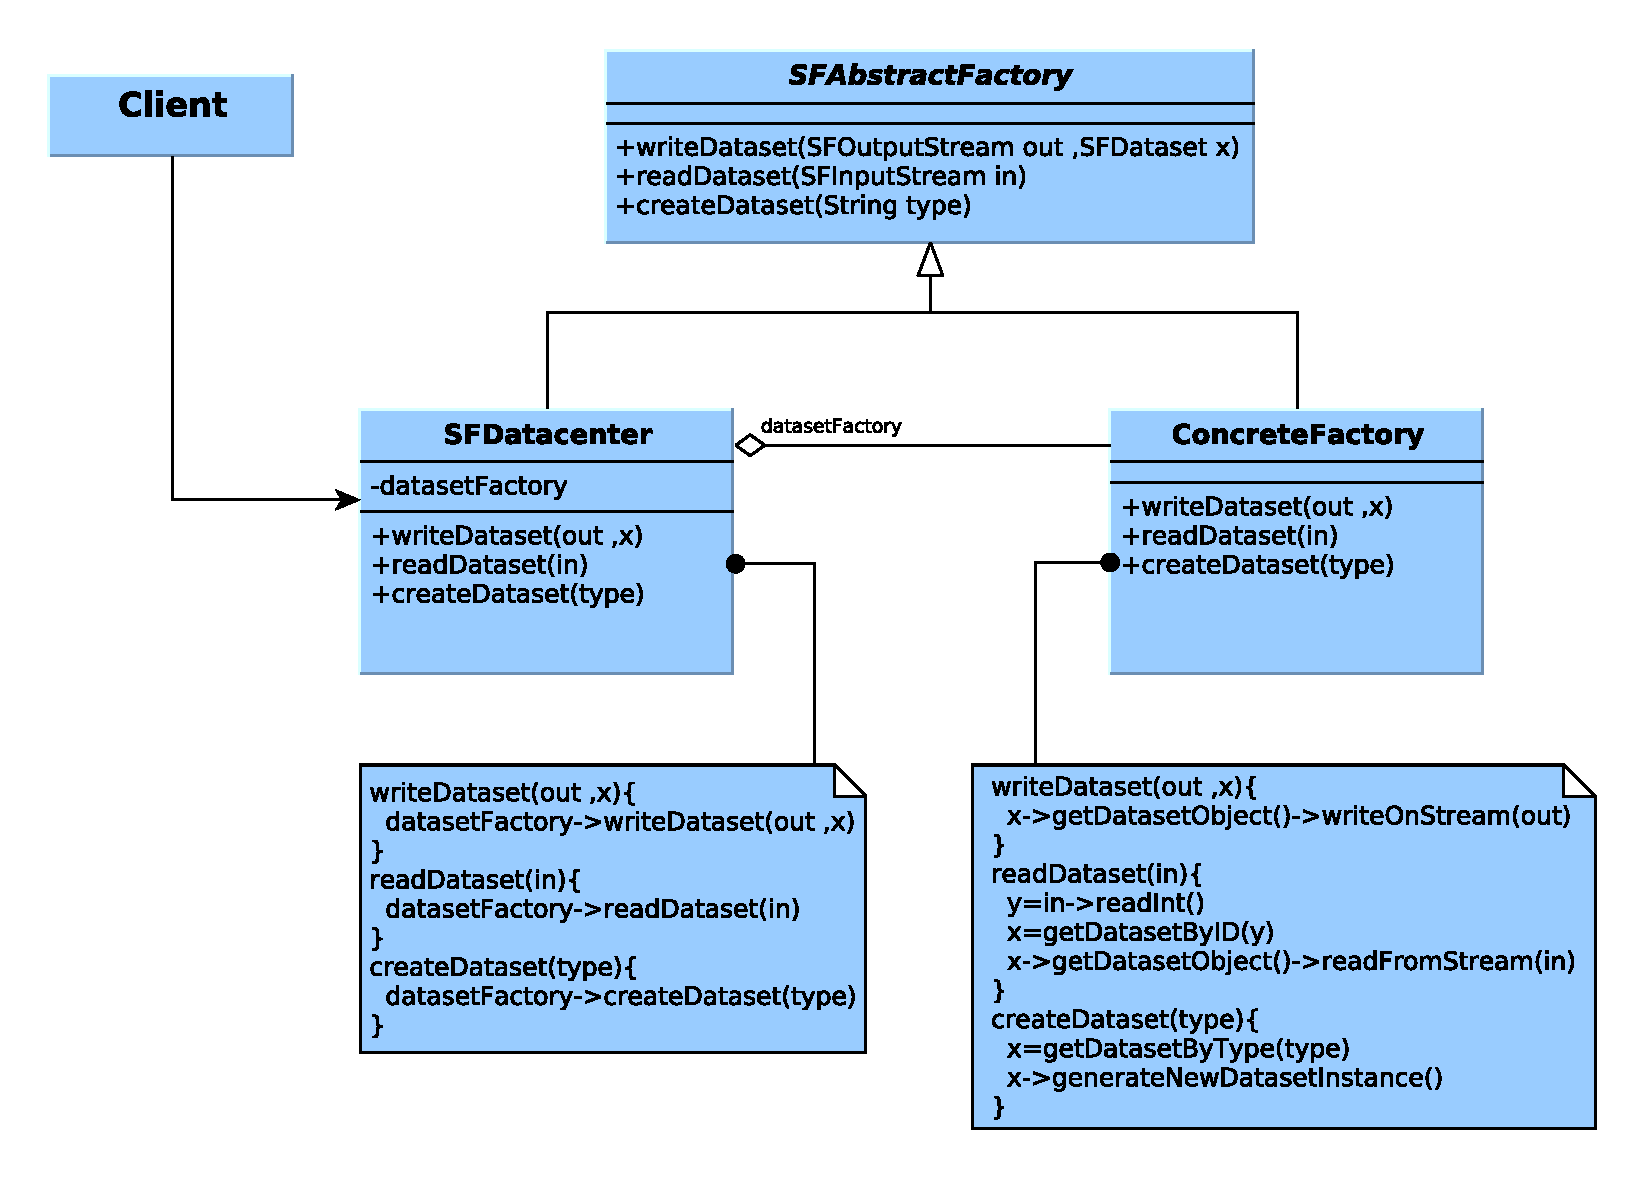
\includegraphics[width=\textwidth]{Immagini/DataCenterfactory}
\caption[Bridge composto da SFDataCenter e SFAbstractFactory]{Diagramma del Bridge composto da SFDataCenter e da un'istanza concreta di SFAbstractFactory.\label{f:datacenterfactory}} 
\end{center} 
\end{figure}
\begin{figure}
\begin{center}
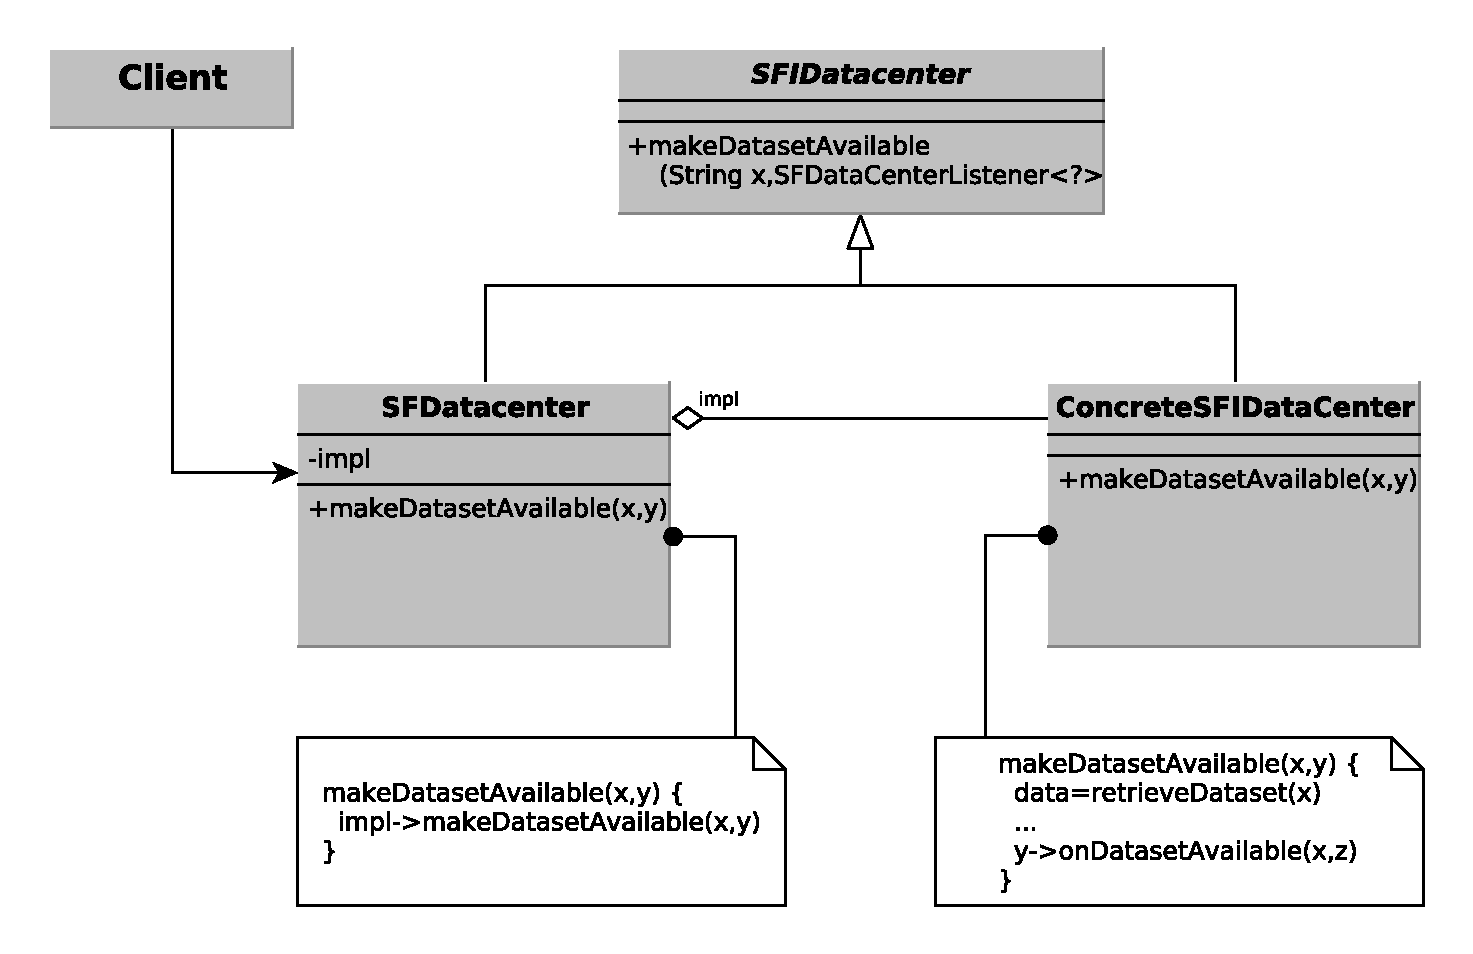
\includegraphics[width=\textwidth]{Immagini/DataCenter}
\caption[Bridge composto da SFDataCenter e SFIDataCenter]{Diagramma del Bridge composto da SFDataCenter e da un'istanza concreta di SFIDataCenter.\label{f:datacenterimplementation}} 
\end{center} 
\end{figure}

\section{Il package \texttt{shadow.system.data}}
\label{sec:shadow_system_data}
Questo package contiene una serie di classi ed interfacce su cui si basa l'astrazione dei dati del framework.

\subsection{SFInputputStream e SFOutputStream}
\label{sub:sfinoutstream}
Queste interfacce definiscono le operazioni necessarie che uno stream di input o di output deve implementare affinch\'e sia possibile leggere o scrivere su di esso dei DataObject e insieme costituiscono un elemento molto importante per l'estendibilit\`a del framework sui dati. Su di esse si basa infatti l'astrazione che i dati utilizzano per completare le operazioni di lettura e scrittura. Utilizzando la medesima interfaccia di astrazione \`e possibile far comunicare tra loro anche implementazioni diverse del framework.

\subsection{SFDataObject}
\label{sub:sfdataobject}
Uno dei moduli principali del package \`e \texttt{SFDataObject}, che rappresenta un'interfaccia con funzionalit\`a di base comuni ad ogni oggetto che contiene dati. 
Ogni oggetto di questo tipo pu\`o perci\`o:
\begin{itemize}
	\item essere scritto su di un \texttt{SFOutputStream};
	\item essere letto da un \texttt{SFInputStream};
	\item essere clonato;
\end{itemize}
I DataObject si basano sul \textit{Composite Pattern}\ref{sub:composite}: possono essere semplici o contenere un insieme di oggetti figli, il fatto che sia gli oggetti complessi che gli oggetti semplici condividano la stessa interfaccia permette di trattare gli oggetti in modo uniforme. Un oggetto contenitore dovr\`a semplicemente richiamare lo stesso metodo di interfaccia per tutti gli oggetti figli i quali, se oggetti semplici, hanno la responsabilit\`a di implementare l'algoritmo per leggere o scrivere se stessi da uno stream.

Tutti i componenti SF utilizzano dei DataObject per incapsulare i dati in modo che questi ultimi possano essere letti e scritti utilizzando stream appropriati.

\begin{figure}
\begin{center}
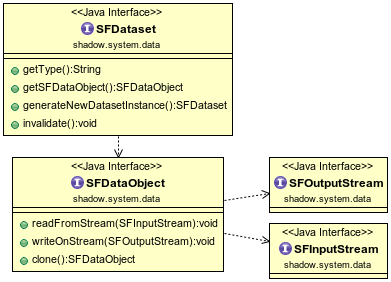
\includegraphics[width=11cm]{Immagini/relazione-dataset-dataobject-stream}
\caption{Diagramma della relazione tra le classi SFDataset, SFDataObject, SFInputStream e SFOutputStream.\label{f:dataset-dataobj-stream}} 
\end{center} 
\end{figure}

\subsection{SFDataset}
\label{sub:sfdataset}
Un altro modulo importante per la gestione dei dati \`e \texttt{SFDataset}. Un Dataset \`e un oggetto che contiene un DataObject e informazioni sul proprio tipo, rappresentato tramite una stringa.
Da come si pu\`o intuire dalla figura \ref{f:dataset-dataobj-stream} il DataObject viene sfruttato dal Dataset per incapsulare i suoi dati interni ed incorporarne le funzionalit\`a di lettura e scrittura.
L'interfaccia SFDataset definisce un'interfaccia per oggetti di questo tipo, la quale consente di accedere al nome del tipo specifico, al DataObject contenuto e di creare una nuova istanza delle stesso tipo.
A loro volta i Dataset possono essere incapsulati in un DataObject usando un oggetto \texttt{SFDatasetObject}.

\subsection{SFAbstractDatasetFactory}
\label{sub:sfabstractdatasetfactory}
Questa interfaccia definisce le operazioni base richieste ad una DatasetFactory, queste operazioni consistono in:
\begin{itemize}
	\item lettura/scrittura di un Dataset da uno stream
	\item la creazione di una nuova istanza di un Dataset specificato per tipo
\end{itemize}

\subsection{SFIDataCenter}
\label{sub:sfidatacenter}
L'interfaccia \texttt{SFIDataCenter} fornisce l'astrazione di una Mappa di Dataset identificati attraverso il proprio nome, attraverso di essa possiamo chiedere di recuperare un Dataset ad un oggetto che la implementa.
Quest'oggetto non deve restituire direttamente il Dataset recuperato, ma deve farlo attraverso un meccanismo di callback ad una implementazione dell'interfaccia \texttt{SFDataCenterListener} passata come parametro, nel momento in cui il dato \`e disponibile.

\begin{figure}
\begin{center}
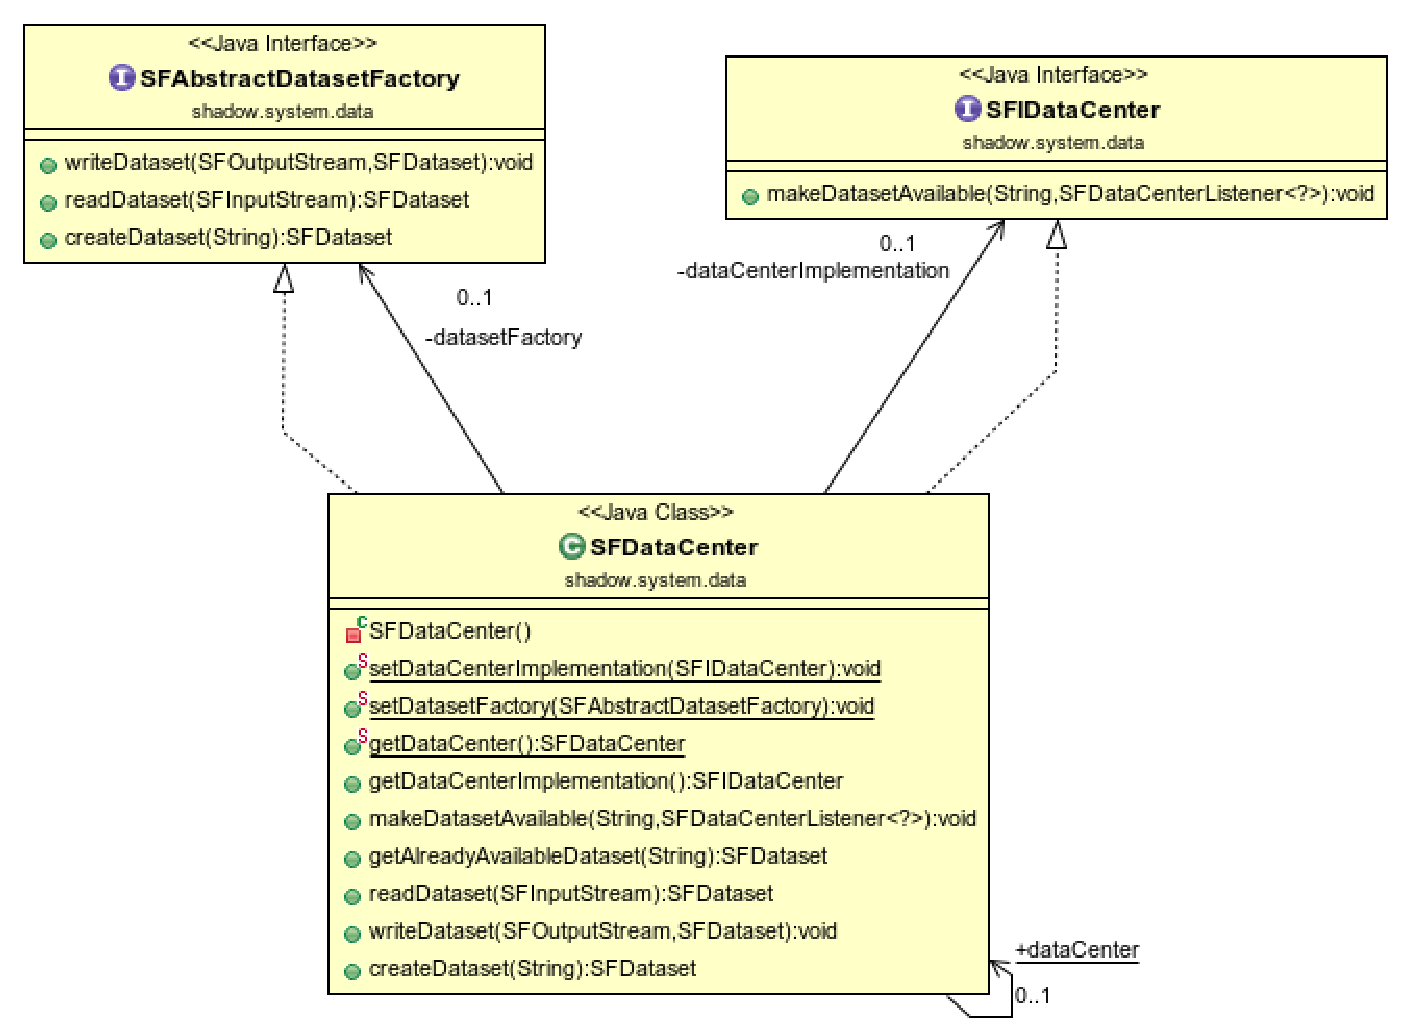
\includegraphics[width=\textwidth]{Immagini/DataCenterBridge}
\caption[Diagramma delle classi di SFDataCenter,SFIDataCenter e SFAbstractDatasetFactory]{In questo diagramma viene mostrata la relazione tra le classi SFDataCenter, SFIDataCenter e SFAbstractDatasetFactory. Da notare che SFDataCenter \`e una classe Singleton in quanto contiene una istanza statica di se stessa (l'istanza dataCenter sottolineata) e possiede un costruttore privato (evidenziato in rosso). Inoltre, in riferimento alla sezione \ref{sub:bridge}, si pu\`o notare come SFDataCenter realizzi un Bridge sia con SFIDataCenter che con SFAbstractDatasetFactory \label{f:datacenterbridge}} 
\end{center} 
\end{figure}

\subsection{SFDataCenterListener}
\label{sub:sfdatacenterlistener}
Questa interfaccia definisce la callback che un componente deve implementare per effettuare una richiesta al DataCenter.
Questa callback viene richiamata quando il Dataset richiesto \`e pronto.

\subsection{SFDataCenter}
\label{sub:sfdatacenter} 
% TODO: evitare di ripetere quanto detto in sec:astrazione
Il \textbf{DataCenter} \`e il nodo fondamentale della gestione dei dati all'interno del framework. 

\'E un oggetto \textit{Singleton} (\ref{sub:singleton}) a cui le applicazioni accedono per richiedere i Dataset di cui hanno bisogno. Questa classe utilizza anche il pattern \textit{Bridge} (\ref{sub:bridge}) per fornendo un'astrazione su come i dati sono effettivamente reperiti.

Per poter funzionare, al DataCenter deve essere fornita un'implementazione per:
\begin{itemize}
	\item \texttt{SFAbstractDatasetFactory}
	\item \texttt{SFIDataCenter}
\end{itemize}

Come precedentemente esposto, l'implementazione di \texttt{SFAbstractDatasetFactory} deve essere essere una factory in grado di generare istanze di tutti i tipi di Dataset necessari all'applicazione.

Questo tipo di astrazione permette di separare la logica di utilizzo del Dataset da quella di come esso viene reperito, consentendo ad una applicazione di usare dati locali o dati di rete semplicemente cambiando l'implementazione di \texttt{SFIDataCenter}.

\subsection{SFObjectsLibrary}
\label{sub:sfobjectslibrary}
\'E usata per memorizzare un set di Dataset ed al suo interno ogni elemento \`e identificato tramite un nome univoco.
Un \texttt{SFObjectsLibrary} \`e a sua volta un Dataset, cos{\`\i} che un ObjectsLibrary possa essere contenuta in altre ObjectsLibrary.
\'E possibile, ad esempio, utilizzare una ObjectLibrary all'interno di implementazione di \texttt{SFIDataCenter} per creare una mappa di Dataset necessari al funzionamento di un'applicazione.

\section{Classi di utilit\`a per il layer dati}

\subsection{SFLibraryreference}
\label{sub:sflibraryreference}
Un LibraryReference \`e un DataObject che pu\`o essere usato da qualsiasi componente per avere un riferimento ad un Dataset memorizzato in una libreria. Viene utilizzato all'interno di DataObject o di Dataset per non avere istanze doppie dello stesso dato.

\subsection{SFGenericDatasetFactory}
\label{sub:sfgenericdatasetfactory}
Questa classe di utilit\`a consiste in una implementazione concreta di default dell'interfaccia \texttt{SFAbstractDatasetFactory}.
Per consentire il riutilizzo del codice questa implementazione sfrutta il meccanismo di \textit{factory con prototipo}: una \textit{factory} pura deve avere un metodo specifico per ogni tipo di oggetto che pu\`o istanziare, questo rende predeterminato il numero di tipi istanziabili e rende necessario modificare il codice, aggiungendo un nuovo metodo, quando si desidera modificare le capacit\`a della \textit{factory}. Una che invece sfrutta il meccanismo dei prototipi non ha un numero predeterminato di tipi istanziabili perch\`e \`e configurabile: attraverso un metodo apposito vengono passati come parametro i prototipi di ogni oggetto che la \textit{factory} deve essere in grado di creare.
Questo sposta la responsabilit\`a dalla conoscenza di come ogni singolo oggetto deve essere allocato sull'oggetto stesso, evitando di dover andare a modificare la \textit{factory} ogni volta che un oggetto viene modificato.
Nel concreto la \texttt{SFGenericDatasetFactory} \`e resa configurabile tramite l'aggiunta di un metodo addSFDataset() consente di generare, in un oggetto GenericDatasetFactory, un elenco di Dataset istanziabili.
Quando verranno chiamati i metodi dell'interfaccia SFAbstractDatasetFactory sull' oggetto GenericDatasetFactory diviene sufficiente richiamare il metodo \texttt{generateNewDatasetInstance()} del Dataset del tipo richiesto.
%!TEX root = ../tesi.tex

\chapter{Il Progetto SF-Remote-Connection}
\label{ch:sfremoteconnection}
In questo capitolo viene descritto il progetto sf-remote-connection, i moduli che lo compongono, le funzionalità offerte e i package java prodotti.

% TODO: trovare un posto per queste info
Il progetto SF-Remote-Connection è una libreria di classi java ospitate, al momento della scrittura di questo documento, sul portale % TODO: aggiungere stile per link
code.google.com per la condivisione di codice open source.

% TODO: cambiare titolo?
\section{Moduli} 
\label{sec:moduli}
La classi che compongono il progetto sono suddivise in una serie di package. % TODO: decidere se la prossima frase va bene
Alcuni di questi sono pensati per rappresentare una possibile estensione a quelli forniti dal framework stesso e ne riproducono la struttura e le convenzioni sui nomi, gli altri invece affiancano o utilizzano il framework nella costruzione dell'applicazione.
Questi package possono perciò essere raggruppati in una serie di macro-moduli suddivisi per funzionalità e finalità:
% TODO: decidere se rinominare i moduli
\begin{enumerate}
	\item \textbf{Base Communication}
	\item \textbf{RemoteDataCenter Tool}
	\item \textbf{Client}
	\item \textbf{Test Client}
	\item \textbf{Server}         
	\item \textbf{Test Server}
\end{enumerate}

% TODO: 
%	inserire un'immagine di come i moduli funzionino su vari livelli
%	verificare i nomi dei package

\subsection{Base Communication}
\label{sub:basecommodule}
Questo modulo riunisce le classi che consentono la creazione e la gestione di connessioni TCP/IP tra applicazioni client/server. Ne fa parte anche la classe di utilità \texttt{GenericCommunicator} che oltre a consentire la gestione della connessione assegnatagli la utilizza per fornire funzionalità di lettura e scrittura di messaggi testuali attraverso il canale aperto.
Il modulo è composto dal package \texttt{sfrc.base.communication} ed è una libreria totalmente indipendente dal framework.

\subsection{RemoteDataCenter Tool}
\label{sub:remotedatacentertoolmodule}
Questo modulo raggruppa una serie di classi pensate per essere una estensione del framework e per essere utilizzate principalmente all'interno di una applicazione client.
La sua funzione principale consiste nel fornire un ponte tra l'astrazione del reperimento dati fornita dal framework e il meccanismo di effettivo reperimento dei dati.

La classe chiave del modulo è \texttt{SFRemoteDataCenter}: le richieste di Dataset effettuate al DataCenter vengono passate a questa classe che le esamina verificando che il dato richiesto sia presente nella libreria dell'applicazione. Se il Dataset non è presente, al richiedente è restituito un Dataset sostitutivo temporaneo scelto opportunamente, contemporaneamente viene generata una richiesta e aggiunta ad un buffer di richieste, questo può essere utilizzato da un modulo esterno in grado di effettuare l'effettivo reperimento dei dati.
% TODO: decidere se i 2 package aggiuntivi andrebbero inseriti nel modulo
Il modulo è composto dai package \texttt{shadow.system.data.remote.wip}, \texttt{shadow.system.data.object.wip} e \texttt{shadow.renderer.viewer.wip}.

\subsection{Client}
\label{sub:clientmodule}
Questo modulo raggruppa tutte quelle componenti generiche che possono essere utilizzate all'interno di una qualsiasi applicazione client e che servono ad implementare l'effettivo reperimento dei dati. 
Esso si pone al di sotto del modulo \textbf{RemoteDataCenter Tool} ed utilizza il modulo \textbf{Base Communication} per la gestione del canale di comunicazione e la sua implementazione è pensata per il multi-threading.
Il package che compone questo modulo è \textbf{sfrc.application.client}.

\subsection{Test Client}
\label{sub:tclientmodule}
In questo modulo sono raccolte le implementazioni test

\subsection{Server}
\label{sub:servermodule}
\subsection{Test Server}
\label{sub:tservermodule}
%!TEX root = ../tesi.tex

\chapter{Test e Risultati}
\label{ch:testerisultati}
Dopo aver definito nel precedente capitolo la struttura del progetto, vengono qui presentati i test effettuati ed i risultati ottenuti.


\section{Test Client}
\label{sec:tclientmodule}

\textbf{Test Client}

In questo modulo sono raccolte le implementazioni delle applicazioni di test per le componenti lato client. Questi test sono stati creati principalmente per riprodurre quelli già presenti nel progetto % TODO: aggiungere riferimento online
SF20LiteTestWorld e usati per mostrare le capacità del framework.
Ne fanno parte anche le classi che implementano i task del protocollo di comunicazione lato client, per la cui trattazione fare riferimento alla sezione \ref{sub:comprotocol}.

Il package che compone questo modulo è \texttt{sfrc.application.client.test} e e \texttt{sfrc.application.client.task}.



\section{Test Server}
\label{sec:tservermodule}

\textbf{Test Server}

Di questo modulo fanno parte le implementazioni di server e applicazioni di test utilizzati per verificare il comportamento delle componenti lato server. Oltre a queste vengono usati per testare i client in differenti condizioni di comunicazione simulate dai server, come ad esempio una risposta a singhiozzo, ecc.
Ne fanno parte anche le classi che implementano i task del protocollo di comunicazione lato server, fare riferimento alla sezione \ref{sub:comprotocol} per una trattazione più approfondita.

Di questo modulo fanno parte i package \texttt{sfrc.application.server.test} e \texttt{sfrc.application.server.task}.




%!TEX root = ../tesi.tex

\chapter{Conclusioni}
\label{ch:conclusioni}
L'obbiettivo del progetto di tesi \`e stato quello di progettare e produrre una serie di moduli software di supporto per lo sviluppo di applicazioni di grafica tridimensionale orientate al Web, che fanno uso dello Shadow Framework. I moduli prodotti si sono dimostrati efficaci allo scopo, consentendo di riprodurre i test effettuati con dati grafici in locale anche nella condizione in cui i dati sono memorizzati su di un server remoto. 
Per consentire la parallelizzazione delle richieste sono stati affrontati numerosi problemi di sincronizzazione per cui \`e stato di fondamentale importanza acquisire familiarit\`a la programmazione multi-thread in Java.


Il lavoro di progettazione e sviluppo del codice \`e stato guidato dai principi di riutilizzo e modularit\`a, sfruttando pratiche quali i \textit{Design Pattern} e le metodologie di sviluppo agile.



\section{Sviluppi futuri}
I possibili sviluppi futuri del lavoro compiuto durante questa tesi sono molteplici e orientati in diverse direzioni, innanzitutto vi \`e la possibilit\`a di espandere i moduli \textbf{Client} e \textbf{Server} in modo che al loro interno vi siano delle utilit\`a per gestire in modo pi\`u completo le sessioni di comunicazione. Con questo si intende la possibilit\`a di instaurare una comunicazione non legata strettamente alle richieste di dati, ma orientata allo scambio di messaggi di controllo, in previsione della possibilit\`a di consentire l'interazione di utenti differenti che condividono la stessa simulazione.

Un'altra possibilit\`a di sviluppo consiste nell'integrare nel modulo \textbf{Base Communication} lo sfruttamento di protocolli di comunicazione pi\`u complessi e potenti, come ad esempio il protocollo peer-to-peer sfruttato nella tesi \cite{tesi:truzzi}.

La possibilit\`a di editare via xml le liste di sostituzione dei dataset non eliminano il problema che la loro produzione sia un lavoro lungo e laborioso, soprattutto quando gli scenari diventano ricchi di modelli tridimensionali. Per questo motivo sarebbe necessario un tool in grado di esaminare i file che descrivono gli scenari e che sia capace di generare in automatico la lista.

\`E in fase di realizzazione un'estensione del protocollo di comunicazione che consenta al server di rispondere alle richieste con una libreria contenente un insieme di Dataset.

Oltre agli sviluppi direttamente collegati al progetto di tesi, i test effettuati hanno evidenziato una serie di elementi del framework che potrebbero avere la necessit\`a di correzioni.

% TODO: eliminare i dettagli ed espandere il generico.

%!TEX root = ../tesi.tex

% NOME PROVVISORIO
\chapter{SFRemoteConnection}
\label{ch:sfremoteconnection}
Appunti sparsi sul progetto

% cambiare il discorso
\section{Obbiettivo del progetto}
\label{sec:obbiettivo}
L'obbiettivo del progetto di tesi nasce dall'idea di produrre un'applicazione dimostrativa della capacit\`a del framework di funzionare con dati residenti su di una macchina remota raggiungibile tramite rete.
L'applicazione che si voleva ottenere era una coppia client-server in cui il server fosse in grado di gestire connessioni simultanee da parte di un numero indefinito di client. 
Ogni client, ottenuta una connessione con il server, doveva assere in grado di visualizzare una scena iniziale navigabile, richiedendo solamente i dati relativi all'ambiente in prossimit\`a di un eventuale avatar.
Successivamente si voleva analizzare due possibili approcci: uno in cui, secondo le necessit\`a, il client avrebbe richiesto al server i dati aggiuntivi riguardo la scena, ad esempio una volta raggiunti i bordi dell'ambiente, oppure un secondo in cui il server, comunicando attivamente con il client, tiene traccia degli spostamenti nella navigazione e fosse in grado di comporre in modo dinamico dei pacchetti di dati prevedendo le necessit\`a del client.

Le astrazioni del layer dati del framework sono state progettate specificatamente per consentire lo sfruttamento della comunicazione di rete, ma fino a quel momento non era stata fatta alcuna specifica implementazione che la utilizzasse. Si desiderava perci\`o produrre questo tipo di applicazione anche per individuare e correggere i probabili bug presenti nel codice e dovuti a vincoli di sincronizzazione ancora non affrontati dato che fino a quel momento tutti i test erano stati effettuati con dati sulla macchina locale.

L'obbiettivo della tesi \`e cos{\`\i} diventato quello di produrre appunto un'implementazione delle astrazioni del framework che utilizzasse la comunicazione di rete per reperire i dati da visualizzare.

% cambiare titolo
\subsection{Infrastruttura di rete} 
\label{sub:rete}
Date le specifiche iniziali \`e stato necessario stabilire quali componenti fosse necessario sviluppare ed in quale ordine. 
Come prima cosa si \`e stabilito di sviluppare una serie di test che replicassero quelli gi\`a funzionanti in locale, per poter fare questo era necessario creare innanzitutto una infrastruttura per la comunicazione di rete tra client e server.

Se da lato client \`e ovvia la necessit\`a di sviluppare uno strato dell'applicazione che si occupasse della comunicazione di rete, da lato server si presentano diverse possibilit\`a: 
\begin{enumerate}
	\item  utilizzare un file server che permettesse semplicemente di accedere ai file contenti i dati tramite la rete;
	\item  utilizzare un application server java, come Tomcat o Glassfish, a cui un'applicazione client potesse connettersi e che attraverso l'esecuzione di servlet realizzasse il trasferimento dei dati da server a client;
	\item  utilizzare un'applicazione server ad hoc appositamente sviluppata;
\end{enumerate}

La prima soluzione \`e probabilmente la pi\`u semplice, ma la meno flessibile dato che consente solo di un accesso diretto ai file di descrizione dei dati senza alcuna possibilit\`a di un'elaborazione lato server e spostando tutto il peso di un'eventuale interazione tra client direttamente su quest'ultimi.

La seconda soluzione offre pi\`u possibilit\`a e flessibilit\`a rispetto alla prima: l'utilizzo di un application server java mette a disposizione una piattaforma che consente una pre-elaborazione dei dati lato server e che possiede direttamente una serie di componenti per la gestione di compiti complessi legati alle sessioni degli utenti, come ad esempio l'autenticazione e la sicurezza. Nonostante i pregi, questo tipo di soluzione possiede anche lati negativi: gli application server generici non sono sviluppati per questo tipo di applicazioni e non era garantita una flessibilit\`a sufficiente per cui all'aumentare della complessit\`a del progetto e delle sue esigenze non fosse necessario abbandonare l'architettura. 

La terza soluzione \`e sicuramente la pi\`u flessibile ed estendibile dato che, se necessario, consente di modificare direttamente il server per adattarsi alle esigenze dell'applicazione. Lo svantaggio \`e la necessit\`a di dover implementare da zero tutte quelle funzionalit\`a non solo di comunicazione, ma anche di autenticazione o di sicurezza che una soluzione gi\`a pronta potrebbe possedere nativamente.

Nella scelta tra le tre soluzioni hanno pesato prevalentemente la volont\`a di realizzare un'architettura funzionante con la scrittura di meno codice possibile e quella di mantenere una bassa complessit\`a iniziale che non penalizzasse per\`o un'estensione futura delle funzionalit\`a. In quest'ottica la prima soluzione è stata anche la prima ad essere scartata, perché sebbene garantisse un tempo di messa in opera molto basso non consente un'estensione di funzionalità. 
La scelta finale è ricaduta sulla terza soluzione che pur costringendo a rinunciare alle funzionalità avanzate della seconda, elimina difficoltà e tempistiche di una installazione e configurazione dell'application server. Inoltre, limitando inizialmente lo sviluppo a funzionalità di base, è possibile limitare la complessità del codice ad un livello non molto più elevato rispetto alla seconda soluzione.


\section{SFRemoteConnection}
\label{sec:sfremoteconnection}

un'implementazione di \texttt{SFIDataCenter} che reperisse i dati attraverso la rete. 


\section{} 
\label{sec:}








\chapter*{TMP}
\label{tmp}
Pluto
\section{tmp1}
Topolino
\subsection{tmp2}
Paperino
\subsubsection{tmp3}
Qui
\paragraph{tmp4}
Quo
\subparagraph{tmp5}
Qua





%----------------------------------------------------------
%	Appendici
%----------------------------------------------------------


%----------------------------------------------------------
%	Bibliografia - Varie
%----------------------------------------------------------

\end{document}